% Uncomment this line for on-screen presentation
\documentclass[xcolor={dvipsnames}]{beamer}\usepackage{etoolbox}\newtoggle{printable}\togglefalse{printable}

% Uncomment this line for printable slides (disable animations and don't waste ink)
%\documentclass[handout, xcolor={dvipsnames}]{beamer}\usepackage{etoolbox}\newtoggle{printable}\toggletrue{printable}

% Adjust these for the path of the theme and its graphics, relative to this file
%\usepackage{beamerthemeFalmouthGamesAcademy}
\usepackage{../../beamerthemeFalmouthGamesAcademy}
\graphicspath{ {../../} }

% Default language for code listings
\lstset{language=C++,
		morekeywords={each,in}
}

\begin{document}
\title{Psychology of Game Interactions}   
\subtitle{COMP140: Creative Computing Hacking}

\frame{\titlepage} 

\begin{frame}{Lecture Objectives}
	Today's lecture will build upon HCI as both a discipline of study and a discipline of design to address:
	
	\begin{itemize}
		\item A well-known \textbf{theory} about cognition from the area of human-computer interaction.
		\item \textbf{How to apply} the theory to the design of user interfaces for games.
	\end{itemize}
	
	This will be followed up by a sprint review in which you will demonstrate your work-in-progress to your tutor.
\end{frame}

\begin{frame}{Important Notice}
	\begin{columns}[onlytextwidth]
		\begin{column}{0.45\textwidth}
			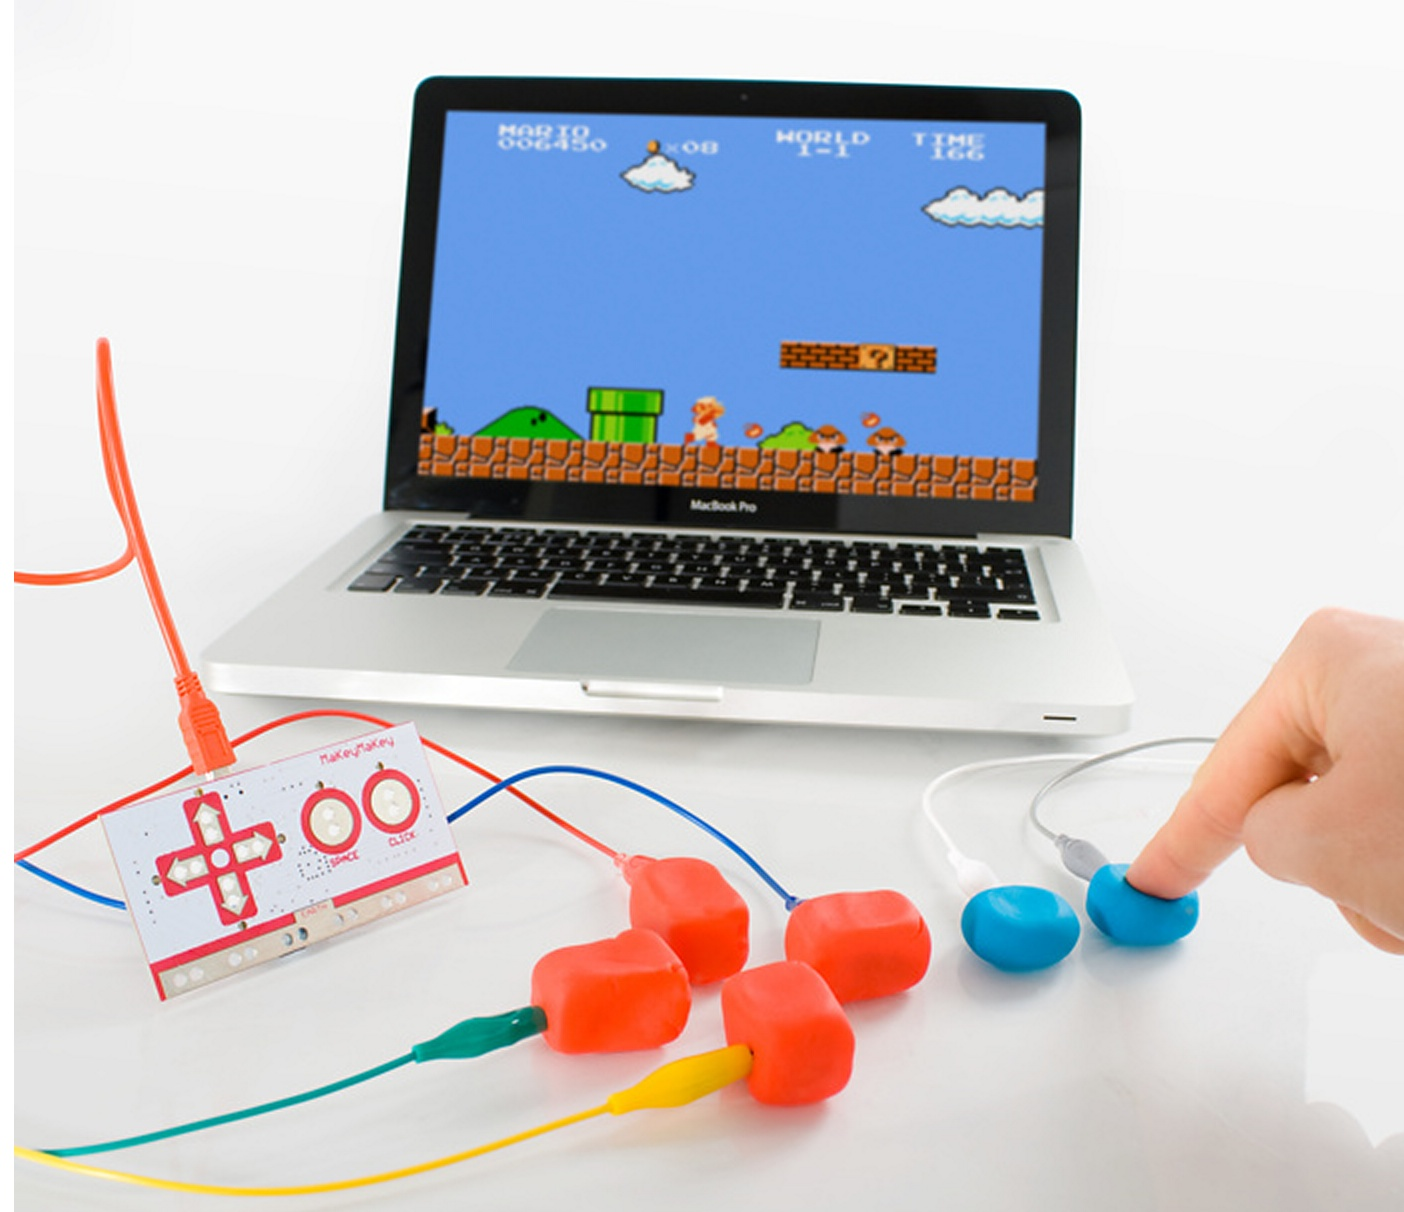
\includegraphics[height=22ex]{MakeyMakey.jpg}
		\end{column}
		\begin{column}{0.45\textwidth}
			Remember to bring your \textit{Makey Makey} kit and associated materials to these lectures for practical 
			support toward the end of each of these sessions.
		\end{column}
	\end{columns}
\end{frame}

\part{Cognition and Information Processing}
\frame{\partpage}

\begin{frame}{Learning Outcomes}
	In this section you will learn how to...
	
	\begin{itemize}
		\item \textbf{Explain} what is meant by `cognition'
		\item \textbf{Show} the importance of information processing models to HCI
		\item \textbf{Explain} the shortcomings of cognitive and information processing models
		\item \textbf{Discuss} the role of cognitive models in games, and HCI more broadly
	\end{itemize}
\end{frame}

\begin{frame}{Further Reading}
	\begin{itemize}
		\item Eysenck, M.W. and Keane, M.T. (2000) \textit{Cognitive Psychology: A Student's Handbook}. 4th Edition. Erlbaum Associatates.
		\item Preece, J., Rogers, Y., Sharp, H., Benyon, D., Holland, S., and Carey, T. (1994) \textit{Human-Computer Interaction}. Addison-Wesley.
	\end{itemize}
\end{frame}

\begin{frame}{What is Cognition?}
	\begin{itemize}
		\item The cognitive approach is currently the dominant framework (or paradigm) for HCI (Perry, 2006).
		\item Players are characterised as `information processors', in which information undergoes a series of ordered processes
		in the player's mind.
		\item This worldview draws a comparison between the human brain and a computer; we can therefore model player activity in the same
		way that we model computer processing.
	\end{itemize}
\end{frame}

\begin{frame}[fragile]{Socrative \texttt{JBYPC3BBY}}
	\begin{itemize}
		\item In pairs.
		\item Quietly discuss what you think is meant by the term `cognition' for 2-minutes.
		\item \textbf{Explain} cognition in your own words.
	\end{itemize}
\end{frame}

\begin{frame}{What is Cognition?}
	\begin{itemize}
		\item Cognition itself refers to the `processes by which we gain knowledge' (Perry, 2006, p. 8).
		
		\vspace{2ex}
		
		\item This includes understanding, remembering, reasoning, attending to, awareness and acquiring skills.
	\end{itemize}
\end{frame}

\begin{frame}{What is Cognition?}
	In a simple model of cognition, such as that proposed by Barber (1988), the process of cognition can be described as composing four sequential
	stages: 
	
	\vspace{2ex}

	\begin{itemize}
		\item Information entering the system as \textbf{input} is first encoded and turned from a physical environment event (i.e., pixels on the screen) 
		into a \textbf{mental representation} held electrochemically in the brain.
		
		\vspace{2ex}
		
		\item This encoded information is then compared to existing repesentations stored in memory.
	\end{itemize}
\end{frame}

\begin{frame}{What is Cognition?}
	In a simple model of cognition, such as that proposed by Barber (1988), the process of cognition can be described as composing four sequential
	stages: 
	
	\vspace{2ex}

	\begin{itemize}
		\item Having compared the representation to the information represented in the memory, the information processor can select an appropriate response.
		
		\vspace{2ex}
		
		\item The final stage involves the execution of the selected response.
	\end{itemize}
\end{frame}

\begin{frame}{What is Cognition?}
	In a simple model of cognition, such as that proposed by Barber (1988), the process of cognition can be described as composing four sequential
	stages: 
	
	\vspace{2ex}

	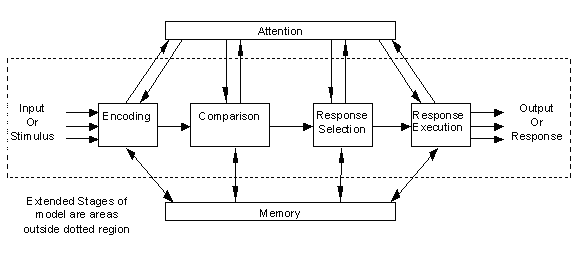
\includegraphics[height=24ex]{barber_cognition.png}
\end{frame}

\begin{frame}[fragile]{Socrative \texttt{JBYPC3BBY}}
	\begin{itemize}
		\item In pairs.
		\item Quietly revisit what is meant by the term `cognition' for 2-minutes.
		\item \textbf{Explain} cognition in your own words.
	\end{itemize}
\end{frame}

\begin{frame}{Cognitve Models in HCI}
	\begin{itemize}
		\item It is important to note that cognitive activity is often conceptualised as being `goal orientated'
		\item This means there is an intended and planned result for the processing.
		\item Or, in other words, `means end analysis' --- determining the difference between the current-state and the goal-state (e.g. interpret current position
		and move towards a power-up, in order to collect it)
	\end{itemize}
\end{frame}

\begin{frame}{Cognitive Models in HCI}
	Newman and Lamming (1995) somewhat controversially called moelling human behaviour in this manner `human virtual machines', drawing from the 
	term `virtual machine', which is a description of an abstract system. 
\end{frame}

\begin{frame}{Cognitive Models in HCI}
	However, as previously illustrated, they have much utility:
	
	\vspace{2ex}

	\begin{itemize}
		\item Understand information requirements needed to identify and progress toward a goal
		\item Optimise representations that are easy for people to encode and compare (e.g. health bar vs absolute number);
		\item Make predictions which can be used to test the efficacy of a design
		\item and so on...
	\end{itemize}
\end{frame}

\begin{frame}{Cognitive Models in HCI}
	Or more generally:
	
	\vspace{2ex}

	\begin{itemize}
		\item Understand what is going on when users use systems
		\item Predict in advance how users will behave
		\item Identify and explain the nature of problems that users encounter
		\item Provide knowledge about what users can and can't be expected to do
		\item Design systems to take advantage of partucular aspects of user skills and abilities
	\end{itemize}
\end{frame}

\begin{frame}{Cognitive Models in HCI}
	There are, however, several drawbacks:
	
	\vspace{2ex}

	\begin{itemize}
		\item An idealised information processing unit is assumed --- people are not so ideal
		\item Individual and ephemeral factors such as motivation and mood play an important role in behaviour;
		\item Considerable variation in characterisitcs and abilities
		\item The system boundary may ignore real-world tools and contexts (e.g. using a DPS calculator instead of performing mental arithmetic manually).
	\end{itemize}
\end{frame}

\begin{frame}[fragile]{Socrative \texttt{JBYPC3BBY}}
	\begin{itemize}
		\item In pairs.
		\item Quietly discuss how cognitive models could inform the design of a game interface.
		\item \textbf{List} the possible uses.
	\end{itemize}
\end{frame}


\part{Variables and types}
\frame{\partpage}

\begin{frame}[fragile]{Variables}
	\begin{columns}[onlytextwidth]
		\begin{column}{0.45\textwidth}
			In Python, variables exist the moment they are assigned to:
			\begin{lstlisting}[language=Python]
a = 10
b = 20
			\end{lstlisting}
			\pause
			Variables can hold values of any type:
			\begin{lstlisting}[language=Python]
a = 10
a = 3.14159
a = "Hello"
			\end{lstlisting}
		\end{column}
		\pause
		\begin{column}{0.45\textwidth}
			In C++, variables must be \textbf{declared} before use, and must be given a \textbf{type}:
			\begin{lstlisting}
int a = 10;
int b = 20;
			\end{lstlisting}
			\pause
			Variables can only hold values of the correct type:
			\begin{lstlisting}
int a = 10;
a = 17;      // OK
a = "Hello"; // Error
			\end{lstlisting}
		\end{column}
	\end{columns}
\end{frame}


\part{Mental Representation \& Conceptual Models}
\frame{\partpage}

\begin{frame}{Learning Outcomes}
	In this section you will learn how to...
	
	\begin{itemize}
		\item \textbf{Define} what is meant by the term `mental model'
		\item \textbf{Explain} the place of mental models in HCI
		\item \textbf{Explain} what a metaphor is
		\item \textbf{Describe} the use of metaphor in HCI
		\item \textbf{Describe} the use of mental models in HCI
	\end{itemize}
\end{frame}

\begin{frame}{Further Reading}
	\begin{itemize}
		\item Lackoff, G. and Johnson, M. (1980) \textit{Metaphors We Live By}. UCP.
		\item Norman, D. and Draper, S. (1986) \textit{User-Centred Systems Design: New Perspectives on Human-Computer Interaction}. LEA.
		\item Norman, D. (1983) `Some Observations on Mental Models' in Gentner and Stevens (eds) \textit{User-Centred Systems Design: New Perspectives on Human-Computer
		 Interaction}. Erlbaum.
		 \item Kempton, W. (1986) \textit{Two Theories of Home Heat Control}, Cognitive Science 10, pp. 75 - 90.
	\end{itemize}
\end{frame}

\begin{frame}{Mental Representation \& Conceptual Models}
	\begin{itemize}
		\item The ways in which information we see, hear, and feel is represented in our brains can have implications for design.
		\item Psychologists believe information is stored so it can be recalled readily.
		\item Topics on knowledge representation include semantic networks, scripts, mental models, and so on---a vast field.
		\item We can leverage these representations through the application of metaphors and conceptual models in designs.
	\end{itemize}
\end{frame}


\begin{frame}{Human Memory Storage}
	\begin{itemize}
		\item Attention and memory are linked --- you remember what you pay attention to (Perry, 2006).
		\item There are three forms of memory store to consider:
		\begin{itemize}
			\item \textbf{very short term sensory store}: iconic; echoic; haptic.
			\item \textbf{mid-term working memory}: commonly referred to as short-term memory.
			\item \textbf{long-term memory}: persistant storage of throughts and ideas.
		\end{itemize}
	\end{itemize}
\end{frame}

\begin{frame}{Human Memory Storage}
	\begin{itemize}
		\item Information moves through sensory to working memory through our attending to it.
		\item Information moves through working memory through rehersal.
	\end{itemize}
\end{frame}

\begin{frame}[fragile]{Socrative \texttt{JBYPC3BBY}}
	\begin{itemize}
		\item In pairs.
		\item An example of long-term memory use in an RTS is remember unit capabilities, while echoic memory might be a confirmation beep when issuing a command.
		\item Quietly discuss other ways we may use memory in an RTS game.
		\item \textbf{Explain ONE} key design decision.
	\end{itemize}
\end{frame}

\begin{frame}{Human Memory Storage}
	There are two sorts of memory usage which we can consider:

	\begin{itemize}
		\item \textbf{recognition}: cues in the environment remind us of things
		\item \textbf{recall}: drawing things from memory without a prompt
	\end{itemize}
\end{frame}

\begin{frame}{Human Memory Storage}
	People find recall more challenging than recognition. Normall (1888) calls these two uses of memory `knowledge in the head' and
	`knowledge in the world', with implications for the ways we use such knowledge:

	\begin{itemize}
		\item as internal representatons (human memory)
		\item from the world through external presentations (memos, events)
		\item embodied in constraints from the world (the limits imposed on our behaviours from the environment
	\end{itemize}
\end{frame}

\begin{frame}[fragile]{Socrative \texttt{JBYPC3BBY}}
	\begin{itemize}
		\item In pairs.
		\item An example of `knowledge in the world' are greyed-out menu items --- users recognise they are not available and do not need to recall this.
		\item Quietly discuss other examples of `knowledge in the world' expressed in a game interface.
		\item \textbf{State ONE} example.
	\end{itemize}
\end{frame}

\begin{frame}{Human Memory Storage}
	Good game interfaces emphasise recognition and knowledge in the world over recall and knowledge in the head.
\end{frame}

\begin{frame}{A Cognitive Economy}
	Nonetheless, there are ways we can improve recall where it is neccessary. Knowledge is organised by people to promote a cognitive economy (Collins \& Quillan, 1969); 
	we do not conduct exhaustive searches of our memory every time we wish to recall something. It is organised in some way.
\end{frame}

\begin{frame}{A Cognitive Economy}
	Two such examples include:

	\begin{itemize}
		\item \textbf{semantic networks}: knowledge is organised by association.
		\item \textbf{scripts}: an encoding of knowledge about a particular context, such that it can guide behaviour.
	\end{itemize}
\end{frame}

\begin{frame}[fragile]{Socrative \texttt{JBYPC3BBY}}
	\begin{itemize}
		\item In pairs.
		\item An example of a semantic network in action is knowing the capabilities of a character based on its class (e.g. a cleric and monk are healers).
		\item An example of a script is knowing what to do to recruit a pick-up group in an MMORPG.
		\item Quietly discuss how semantics and scripts may influence game interaction.
		\item \textbf{Explain ONE} example, \textbf{briefly stating} which concept you are referring to.
	\end{itemize}
\end{frame}

\begin{frame}{Mental Models in Psychology}
	\begin{itemize}
		\item Norman (1983) describes mental models as `mental simulations'; models that people have of themselves, others,the environment, things they interact with, etc.
		\item Remember the fridge example from last week? You may well have developed an incorect mental model while trying to decipher the controls.
	\end{itemize}
\end{frame}

\begin{frame}{Mental Models in Psychology}
	\begin{centering}
		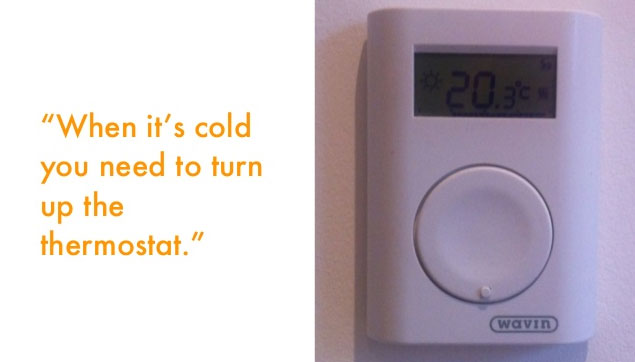
\includegraphics[height=26ex]{thermostat_invalid_model.jpg}
	\end{centering}
	
	\vspace{2ex}
	
	(see Kempton, 1986)
\end{frame}


\begin{frame}[fragile]{Socrative \texttt{JBYPC3BBY}}
	\begin{itemize}
		\item Briefly, is the statement correct?
	\end{itemize}
\end{frame}

\begin{frame}{Mental Models in Psychology}
	\begin{itemize}
		\item We build mental models to predict external events before we take action.
		\item Play an important role in human reasoning, and consequently player behaviour in games.
		\item Are players developing an accurate mental model?
	\end{itemize}
\end{frame}

\begin{frame}{Mental Models in Psychology}
	\begin{centering}
		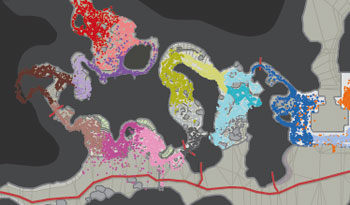
\includegraphics[height=20ex]{halo_heat_map.jpg}
	\end{centering}
	
	\vspace{2ex}
	
	(Thomson, 2007) \\
	\url{http://archive.wired.com/gaming/virtualworlds/magazine/15-09/ff_halo?currentPage=all}
\end{frame}

\begin{frame}{Conceptual Models in the Interface}
	\begin{itemize}
		\item Players need to understand their actions in order to make meaningful choices.
		\item As such, designers need to design an interface in a way that shapes the players' mental model construction.
		\item Normal (1988) suggests how the design and the player's mental model are linked through the `system image' (i.e. the visible part
		of the interactive system).
	\end{itemize}
\end{frame}

\begin{frame}{Conceptual Models in the Interface}
	``In many ways the primary task of designer is to construct an appropriate system image, realising that everything the user interacts with helps us to inform that image:
	the physical knobs, dials, keyboards, and displays [...] text, input, output, and error messages''
	
	\vspace{2ex}
	
	(Normal, 1986, p. 44)
\end{frame}

\begin{frame}{Conceptual Models in the Interface}
	Newman and Lamming (1995) provide design guidelines along these lines:

	\begin{itemize}
		\item Identify the mental model you intend the player to adopt, preferably before designing the game interface;
		\item Link the mental model to the intended means of interaction;
		\item Hide aspects of the system image that conflict with player performance on an action/activity;
		\item Explout the system image to convey the intended mental model;
		\item and show the state of the game as it is \textit{now}---not as it was some time ago.
	\end{itemize}
\end{frame}

% Move this to next week
%\part{Functions}
\frame{\partpage}

\begin{frame}[fragile]{Function definitions}
    \begin{itemize}
        \item We have already seen an example of a function definition
    \end{itemize}
    \begin{lstlisting}
int main()
{
    std::cout << "Hello, world!" << std::endl;
    return 0;
}
    \end{lstlisting}
    \begin{itemize}
        \item The function \lstinline{main} takes no parameters, and returns a value of type \lstinline{int}
    \end{itemize}
\end{frame}

\begin{frame}[fragile]{Function signatures}
    \begin{itemize}
        \item The \textbf{signature} of a function defines its return type, name, and parameters
    \end{itemize}
    \begin{lstlisting}
double foo(std::string x, int y, bool z)
    \end{lstlisting}
    \pause
    \begin{itemize}
        \item This function takes three parameters: \pause
        \lstinline{x} of type \lstinline{std::string}, \pause
        \lstinline{y} of type \lstinline{int}, \pause
        and \lstinline{z} of type \lstinline{bool} \pause
        \item It returns a value of type \lstinline{double}
    \end{itemize}
\end{frame}

\begin{frame}[fragile]{Functions without return values}
    \begin{itemize}
        \item It is possible to define a function which does not return a value, using the \lstinline{void} keyword
        in place of its return type
    \end{itemize}
    \pause
    \begin{lstlisting}
void printNumber(int n)
{
    std::cout << n << std::endl;
}
    \end{lstlisting}
\end{frame}

\begin{frame}[fragile]{Pass by value}
    \begin{itemize}
        \item Function parameters are passed \textbf{by value}:
        the function receives \textbf{copies} of the original variables
    \end{itemize}
    \pause
    \begin{lstlisting}
void changeName(std::string name)
{
    name = "Ed";
}

int main()
{
    std::string name = "Mike";
    std::cout << name << std::endl; // Mike
    changeName();
    std::cout << name << std::endl; // Mike
}
    \end{lstlisting}
\end{frame}

\begin{frame}[fragile]{Pass by reference}
    \begin{itemize}
        \item Parameters can be passed \textbf{by reference} using \lstinline{&}, allowing the function to modify them
    \end{itemize}
    \pause
    \begin{lstlisting}
void changeName(std::string& name)
{
    name = "Ed";
}

int main()
{
    std::string name = "Mike";
    std::cout << name << std::endl; // Mike
    changeName();
    std::cout << name << std::endl; // Ed
}
    \end{lstlisting}
\end{frame}

\begin{frame}[fragile]{One area where C++ is ``simpler'' than Python!}
    \begin{itemize}
        \item Recall from COMP110 week 6: in Python, basic data types (numbers, booleans, strings etc)
            are passed by value, and object types (lists, dictionaries, class instances) are passed by reference
        \pause
        \item In C++, everything is passed by value unless it is explicitly marked as a reference with \lstinline{&}
    \end{itemize}
\end{frame}

\begin{frame}[fragile]{Constant references}
    \begin{lstlisting}
void greet(std::string name)
{
    std::cout << "Hi " << name << std::endl;
}
    \end{lstlisting}
    \pause
    \begin{itemize}
        \item The string will be copied in order to be passed in \pause
        \item More efficient to pass a reference, and mark it \lstinline{const} to prevent accidental modification
    \end{itemize}
    \begin{lstlisting}
void greet(const std::string& name)
{
    std::cout << "Hi " << name << std::endl;
}
    \end{lstlisting}
    \pause
    \begin{itemize}
        \item (this is only worthwhile for large data structures like strings and vectors, not for basic data types)
    \end{itemize}
\end{frame}



\part{Practical Activity}
\frame{\partpage}

\begin{frame}{Sprint Review}
	\begin{itemize}
		\item \textbf{Load} the game you are working with.
		\item \textbf{Connect} your novel game controller.
		\item \textbf{Demonstrate} the prototype to your tutor.
		\item While you are waiting, self-organise into pairs to discuss your work-in-progress. Focus on the psychology
		of the game interface and how psychological concepts could inform the design. Remember, you are assessing the interactivity; 
		not just the controller itself. Be broard and all-encompassing in your discussions.
	\end{itemize}
\end{frame}

\begin{frame}{Coursework Progress}
	\begin{itemize}
		\item \textbf{Continue} developing the prototype.
		\item \textbf{Conduct} some form of play test within the next week.
	\end{itemize}
\end{frame}

% -------------------------------------------------------

%\part{The compiler}
%\frame{\partpage}
%
%\begin{frame}
%	\frametitle{The build process}
%	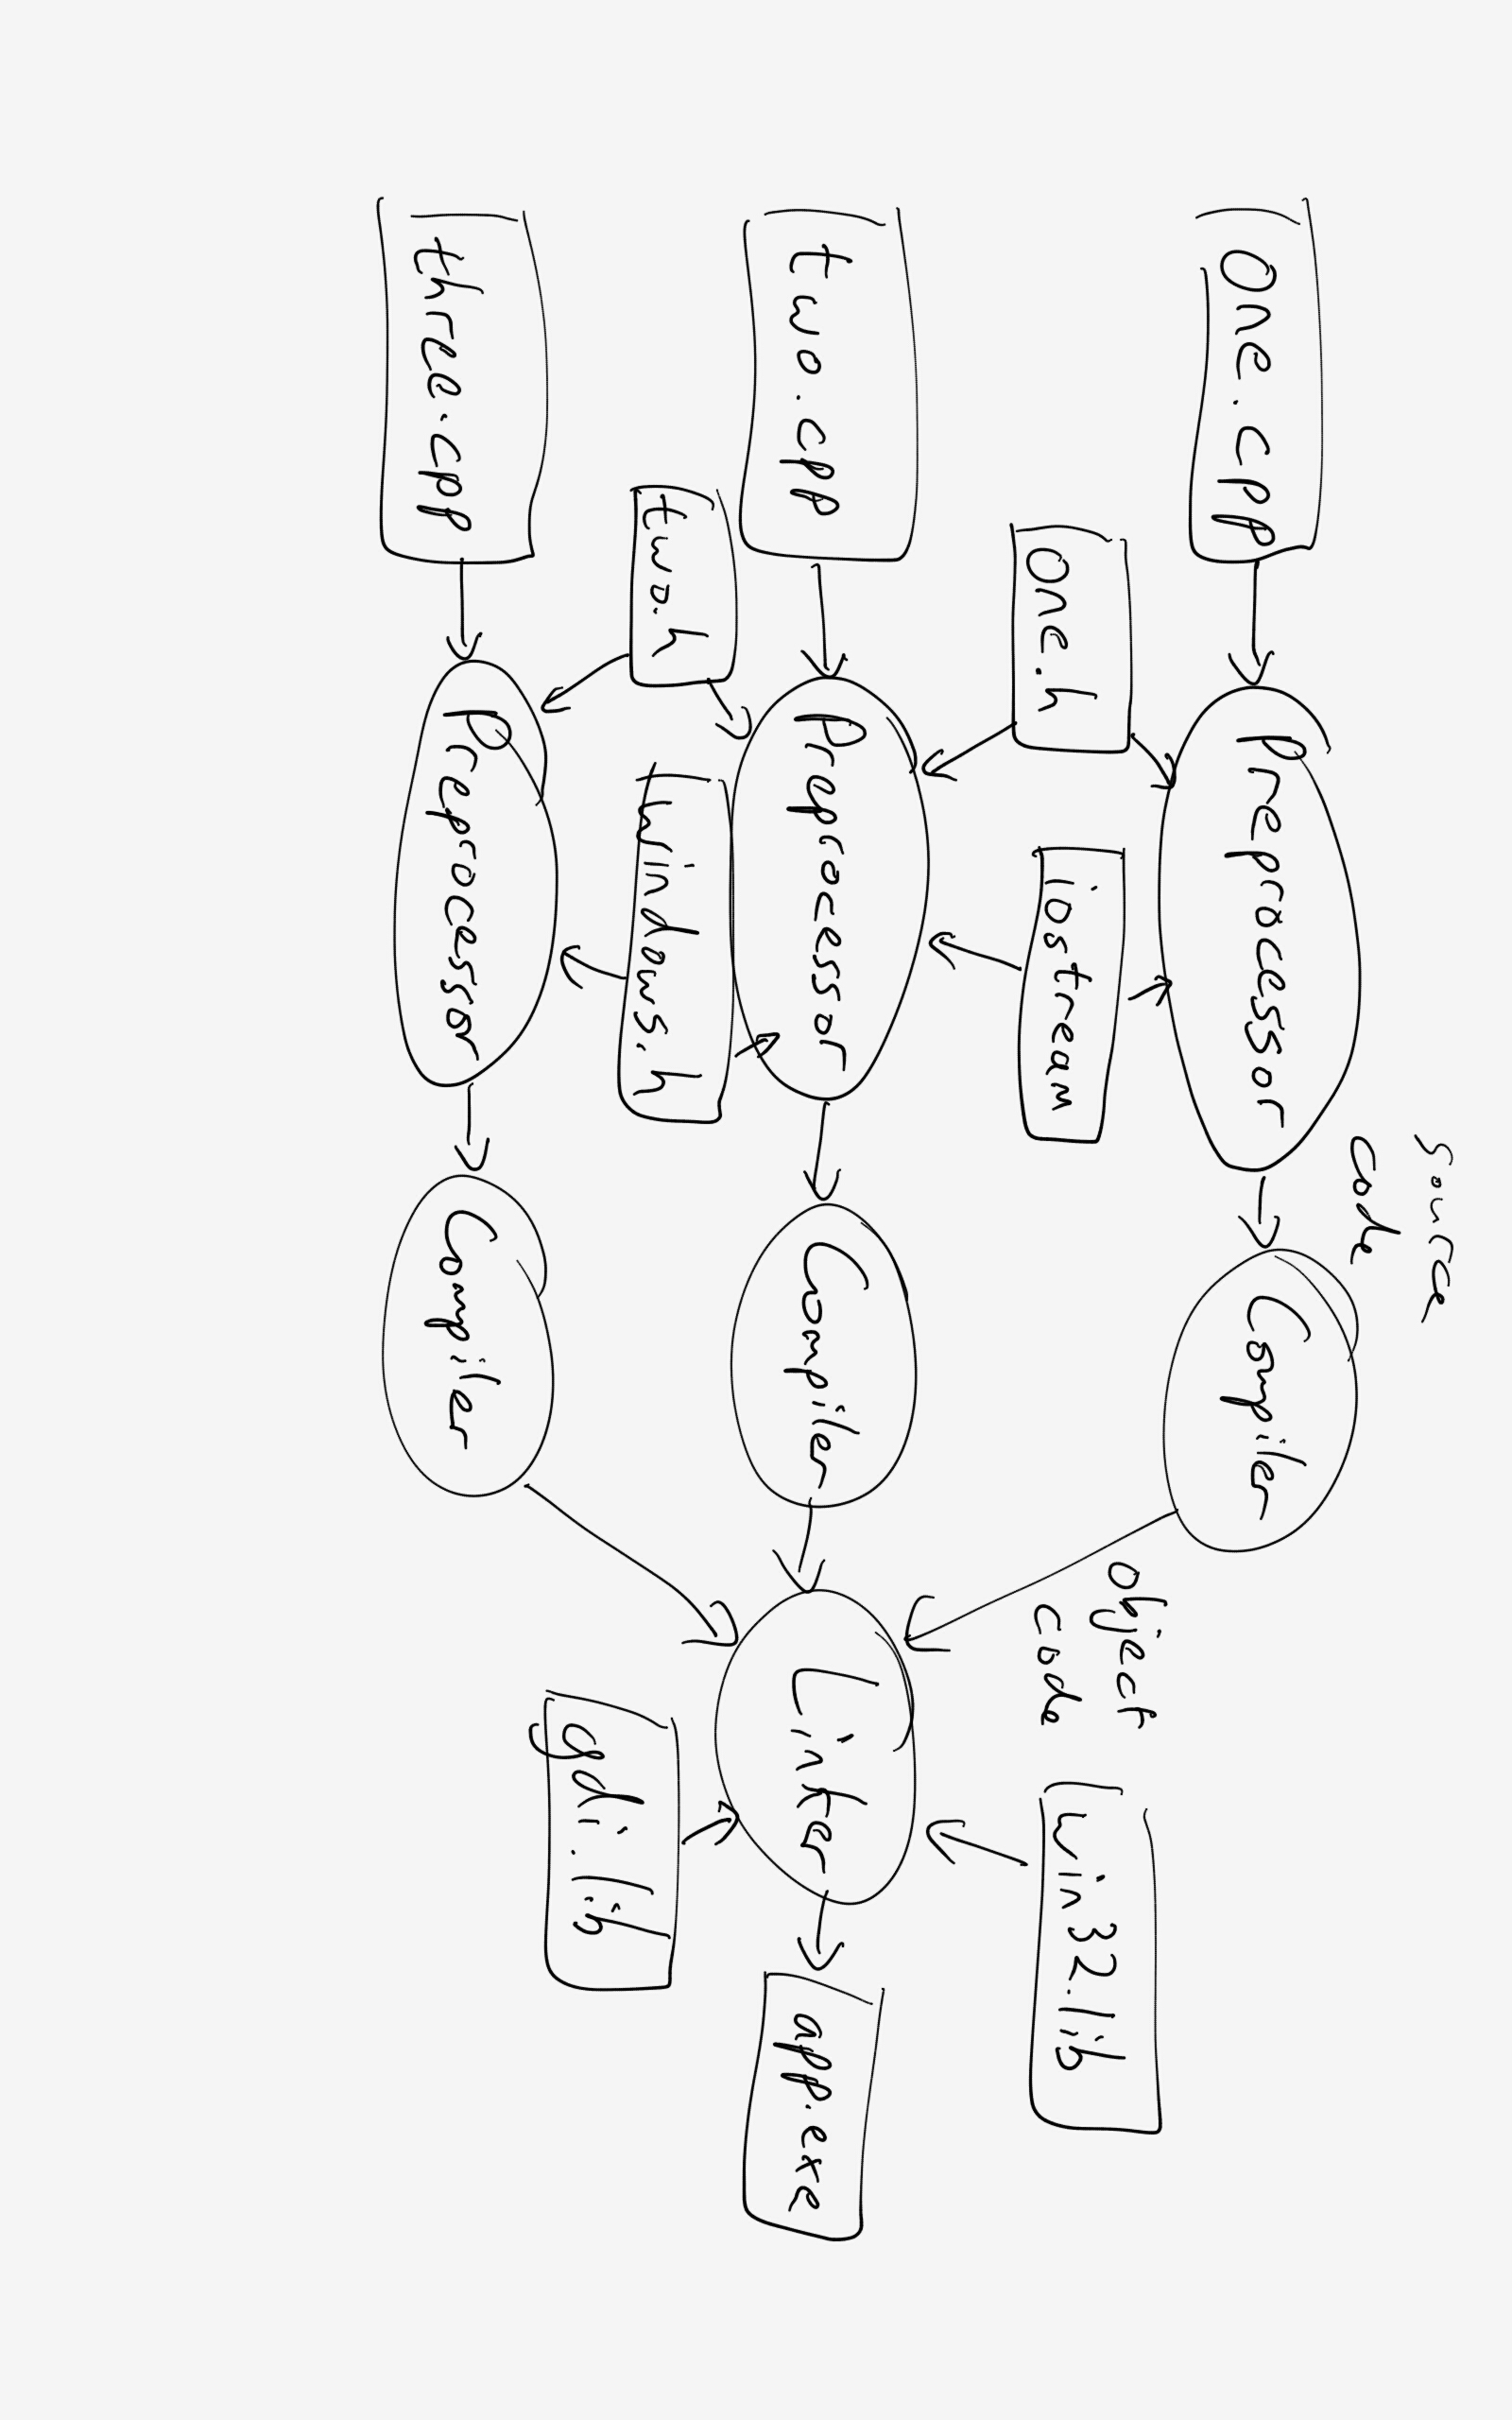
\includegraphics[height=\textwidth,angle=90]{compiler_sketch}
%\end{frame}

\end{document}
